\documentclass[conference]{IEEEtran}
\IEEEoverridecommandlockouts

\usepackage{cite}
\usepackage{amsmath,amssymb,amsfonts}
\usepackage{algorithmic}
\usepackage{algorithm}
\usepackage{graphicx}
\usepackage{textcomp}
\usepackage{xcolor}
\usepackage{booktabs}
\usepackage{multirow}
\usepackage{tikz}
\usetikzlibrary{positioning,arrows.meta,fit,calc,shapes.geometric,decorations.pathreplacing}

\def\BibTeX{{\rm B\kern-.05em{\sc i\kern-.025em b}\kern-.08em
    T\kern-.1667em\lower.7ex\hbox{E}\kern-.125emX}}

\begin{document}

\title{AND-Popcount MLB-MAC: An Energy-Efficient FP8\\
Dot-Product Accelerator for DNN Inference}

\author{
\IEEEauthorblockN{Shreyas S.~Kulkarni}
\IEEEauthorblockA{
IIIT Bangalore\\
ShreyasS.Kulkarni@iiitb.ac.in}
\and
\IEEEauthorblockN{Grover Heer}
\IEEEauthorblockA{
IIIT Bangalore\\
Heer@iiitb.ac.in}
\and
\IEEEauthorblockN{Madhav Rao}
\IEEEauthorblockA{
IIIT Bangalore\\
mr@iiitb.ac.in}
}

\maketitle

% =========================================================================
% ABSTRACT
% =========================================================================
\begin{abstract}
We propose an energy-efficient dot-product accelerator for DNN
inference that replaces conventional FP8 multiplier arrays with
bitwise AND gates and popcount reduction trees, achieving significant
area and power savings.  The design operates natively in the FP8
(E4M3) format and exploits Multi-Level Binary~(MLB) decomposition
combined with Block Floating Point~(BFP) alignment to replace $N$
parallel multipliers with $N$-wide AND gates and a single
$\lceil\log_2 N\rceil$-depth adder tree per bit-plane pair.  Unlike
prior MLB approaches that used XNOR-popcount and required
substantial correction circuitry, our design leverages the inherently
unsigned structure of FP8 mantissas to make AND-popcount
correction-free.  We compare three FP8 dot-product architectures ---
(1)~the proposed AND-popcount MLB-MAC with BFP, (2)~a conventional
integer MAC with the same BFP front end, and (3)~a native FP8 MAC
without BFP blocking --- synthesized on the
45\,nm technology node using the FreePDK45 library, reporting
area, power, and energy efficiency.  A Quantization-Aware Training~(QAT) sweep on
ResNet-20/CIFAR-10 with exponent-sorted blocking across
$N \in \{9, 25, 32, 64, 128, 256, 512\}$ characterises the
accuracy--area trade-off of the BFP-based architectures.
\end{abstract}

\begin{IEEEkeywords}
DNN accelerators, FP8, E4M3, MAC array, AND-popcount, multi-level
binary, block floating point, quantization-aware training, energy
efficiency, RTL verification
\end{IEEEkeywords}

% =========================================================================
\section{Introduction}
% =========================================================================

The dominant computational primitive in deep neural network~(DNN)
inference is the multiply-accumulate~(MAC) operation.  For a single
output neuron, the accelerator computes the dot product
$y = \sum_{k=0}^{K-1} x_k \cdot w_k$, which requires $K$
multiplications and $K{-}1$ additions.  In modern convolutional and
transformer-based networks, $K$ can exceed tens of thousands, making
the MAC array the primary consumer of silicon area and dynamic power.

The 8-bit floating-point format FP8, in particular the E4M3
variant~\cite{b2,b3}, has emerged as a practical balance between
dynamic range and hardware cost for inference.  However, even at
8-bit precision, conventional FP8 MAC designs remain expensive:
each lane requires a mantissa multiplier, per-element barrel
shifters for exponent alignment, and wide reduction trees.

Multi-Level Binary~(MLB) representation offers a fundamentally
different approach~\cite{b1}.  Instead of computing $x_k \cdot w_k$
with an explicit multiplier, MLB decomposes each operand into $M$
binary bit-planes and computes the cross-product terms using
bitwise logic (AND or XNOR) followed by a population count
(popcount).  This replaces $N$ multipliers with $M^2$ instances of
$N$-wide bitwise gates and popcount reduction trees --- structures
that are inherently simpler, lower-power, and smaller in area
than multiplier arrays.

To make this work with FP8 operands, we combine the MLB core with
a Block Floating Point~(BFP) front end that groups $N$ FP8 values
under a shared exponent.  The BFP stage converts each FP8 mantissa
(with hidden bit) into a 4-bit aligned unsigned integer, which can
then be decomposed into $M = 4$ bit-planes that the MLB array
consumes.  This \emph{BFP + MLB} pipeline eliminates all
per-element multipliers from the critical path.  The relationship
between the dot-product size $K$ and the block size $N$ naturally
admits three regimes: when $K = N$, a single BFP block covers the
entire dot product; when $K > N$, the dot product is partitioned
into $\lceil K/N \rceil$ independent blocks, each processed by one
BFP-MLB pass with results summed in software; when $K < N$,
the dot product is zero-padded to~$N$.  We sweep over multiple
$N$ values to characterise these trade-offs.

A key enabler of this design is the observation that FP8~(E4M3)
mantissas --- including the recovered hidden bit --- are \emph{strictly
unsigned} binary fractions.  A logical~0 in any mantissa bit
corresponds exactly to a mathematical~0.  This allows us to use a
plain AND gate (rather than XNOR) as the bitwise core, which
computes $\text{AND}(x_i, x_j) = x_i \cdot x_j$ for
$x_i, x_j \in \{0,1\}$ with no offset.  Prior MLB-MAC work used
XNOR-popcount~\cite{b1}, which introduced a bipolar offset
requiring dedicated correction circuits; for FP8 operands, the
AND-popcount approach eliminates this correction overhead entirely
(see Section~\ref{ssec:xnor_lesson}).

In this paper, we compare three architectures for computing FP8
dot products:
\begin{enumerate}
    \item \textbf{AND-Popcount MLB-MAC + BFP} (proposed):
    Replaces multipliers entirely with AND gates and popcount trees.
    An input time-multiplexing FSM shares a single MLB array
    between positive and negative sign lanes, halving the hardware.
    \item \textbf{Integer MAC + BFP} (Baseline~1):
    Uses $N$ conventional unsigned multipliers with per-lane sign
    handling. Shares the same BFP front end, enabling a fair
    comparison of the MAC core.
    \item \textbf{Native FP8 MAC} (Baseline~2):
    Performs per-element FP8 multiplication with individual exponent
    handling (per-element barrel shifters) and no BFP blocking.  This
    represents the most hardware-expensive approach.
\end{enumerate}

\subsection*{Contributions}
\begin{enumerate}
    \item We propose an AND-popcount MLB-MAC architecture that replaces
    all per-element multipliers with $N$-wide AND gates and
    $\lceil\log_2 N\rceil$-depth popcount trees, combined with a
    BFP front end that amortizes exponent handling across $N$
    elements.
    \item We design a complete parameterizable RTL pipeline ---
    including BFP aligner with corner turn, AND-popcount reduction
    tree, zero-gate-multiplier MLB unit, MLB array, sign-mask FSM
    for time-multiplexed resource sharing, and output combiner ---
    and generate synthesizable Verilog across
    $N \in \{9, 25, 32, 64, 128, 256, 512\}$.
    \item We compare all three FP8 dot-product architectures
    synthesised on the 45\,nm node using the FreePDK45 library,
    reporting area, power, and energy efficiency.
    \item We develop a bit-accurate PyTorch emulator with
    Straight-Through Estimator~(STE)~\cite{b_ste} gradients and
    run a QAT sweep on ResNet-20/CIFAR-10 to characterise the
    accuracy--area trade-off as a function of BFP block size~$N$.
\end{enumerate}

% =========================================================================
\section{Background}
% =========================================================================

\subsection{FP8 E4M3 Number Format}
\label{ssec:fp8}

The FP8 E4M3 format~\cite{b2,b3} encodes each value with one sign
bit~$s$ (bit~7), four exponent bits~$e_{3:0}$ (bits~6:3,
bias~$= 7$), and three explicit mantissa bits~$m_{2:0}$
(bits~2:0).  For normalised values ($e \neq 0$):
\begin{equation}
    \text{value} = (-1)^s \times 2^{e - 7} \times
    \underbrace{(1.m_2 m_1 m_0)_2}_{\text{4-bit unsigned mantissa}}.
    \label{eq:fp8_decode}
\end{equation}
Table~\ref{tab:fp8_special} summarises the E4M3 special values.

\begin{table}[htbp]
\centering
\caption{FP8 E4M3 special value encodings.}
\label{tab:fp8_special}
\footnotesize
\begin{tabular}{lll}
\toprule
Class & Encoding & Value \\
\midrule
Max normal     & \texttt{S.1111.110}$_2$ & $\pm 1.75 \times 2^{8} = \pm 448$ \\
Min normal     & \texttt{S.0001.000}$_2$ & $\pm 2^{-6}$ \\
Max subnormal  & \texttt{S.0000.111}$_2$ & $\pm 0.875 \times 2^{-6}$ \\
Min subnormal  & \texttt{S.0000.001}$_2$ & $\pm 2^{-9}$ \\
Zero           & \texttt{S.0000.000}$_2$ & $\pm 0$ \\
NaN            & \texttt{S.1111.111}$_2$ & N/A \\
\bottomrule
\end{tabular}
\end{table}

Note that E4M3 has no infinities; the encoding
\texttt{S.1111.111}$_2$ is reserved for NaN.  Subnormal values
($e = 0$) are flushed to zero in our hardware, following standard
inference practice.

The critical structural property exploited in this work is that the
4-bit unsigned mantissa $\{1, m_2, m_1, m_0\}$ takes values in
$\{8, 9, \ldots, 15\}$ for normal inputs, with the sign captured
entirely by the dedicated sign bit.  A logical~0 in any mantissa
bit contributes exactly~0 --- there is no bipolar encoding.

\subsection{Block Floating Point}
\label{ssec:bfp}

Block Floating Point~(BFP) reduces the cost of floating-point dot
products by sharing a single exponent across a block of $N$
operands~\cite{b3}.  For each block, the maximum exponent
$e_{\max}$ is identified, and each element is right-shifted by
$\Delta e_k = e_{\max} - e_k$ bits:
\begin{equation}
    m_k^{\text{aligned}} = \lfloor m_k \cdot 2^{-\Delta e_k} \rfloor.
    \label{eq:bfp_align}
\end{equation}
After alignment, all mantissas share the same implicit radix point,
and the dot product reduces to purely integer arithmetic with a
single shared exponent.  This amortizes the costly per-element
barrel shifters of native FP8 designs across $N$ elements, replacing
them with a single max-finder and $N$ fixed-width right shifters.

As $N$ increases, two competing effects arise:
\begin{enumerate}
    \item \textit{Area amortization:} The BFP alignment circuit is
    shared across more elements, reducing per-element overhead.
    \item \textit{Precision loss:} When one element has a much
    larger exponent than the others, the right-shift for the smaller
    elements exceeds 3~bits (the full mantissa width), flushing them
    to zero.  This effect becomes increasingly severe at larger $N$
    as the probability of outlier exponents grows.
\end{enumerate}
We use a QAT sweep across multiple $N$ values and an
exponent-sorting strategy to characterise and mitigate this
accuracy degradation, identifying the Pareto-optimal block size.

\subsection{Multi-Level Binary Representation}
\label{ssec:mlb_bg}

Multi-Level Binary~(MLB) representation~\cite{b1} decomposes a
quantised $M$-bit value $x_q$ into $M$ binary components weighted
by scaling factors $\alpha_i$:
\begin{equation}
    x_q = \sum_{i=1}^{M} \alpha_{x_i} \, s_{x,i},
    \quad s_{x,i} \in \{-1,+1\},
    \label{eq:mlb_repr}
\end{equation}
where $\alpha_{x_i}$ are the scaling factors and $s_{x,i}$ are
the binary-valued components.  For unsigned bit-planes (as in our
FP8 design), $b_i \in \{0,1\}$ with $\alpha_i = 2^{i-1}$, and the
representation simplifies to
$x_q = \sum_{i=0}^{M-1} 2^i \, b_i$.

The dot product of two $K$-element vectors, each decomposed into $M$
planes, can be factored as~\cite{b1}:
\begin{equation}
    \text{dot}(\mathbf{x}_q, \mathbf{w}_q) =
    \sum_{i=1}^{M} \sum_{j=1}^{M} \alpha_{x_i}\,\alpha_{w_j}
    \sum_{k=1}^{K} s_{x_{k,i}}\, s_{w_{k,j}}.
    \label{eq:mlb_dot}
\end{equation}
The inner sum $\sum_{k=1}^{K} s_{x_{k,i}}\, s_{w_{k,j}}$ can be
computed by a bitwise operation (XNOR for bipolar, AND for unsigned)
followed by a popcount over $K$ elements.  When $N$ parallel
operations are employed, a block of $N$ elements is processed
simultaneously.  This replaces $N$ multipliers with $M^2$ instances
of $N$-wide bitwise gates and popcount trees.

For the FP8~(E4M3) mantissa with hidden bit, $M = 4$ planes with
fixed power-of-two scaling factors $\alpha = \{1, 2, 4, 8\}$,
yielding $M^2 = 16$ popcount terms per block.  Since
$\alpha_{x_i} \cdot \alpha_{w_j} = 2^{i+j}$, the scaling reduces
to a static left-shift by $(i+j)$ --- a zero-gate operation.

Following~\cite{b1}, the key design parameters are:
\begin{itemize}
    \item $M$: data width (number of bit-planes per operand); fixed
    at $M = 4$ for FP8.
    \item $N$: parallelism factor (number of elements processed in
    parallel within one BFP block).
    \item $K$: dot-product size (total elements in the inner product).
\end{itemize}
When $K > N$, the dot product is partitioned into
$\lceil K/N \rceil$ blocks.  When $K < N$, the inputs are
zero-padded.

\subsection{The XNOR-Popcount Lesson}
\label{ssec:xnor_lesson}

The original MLB-MAC architecture~\cite{b1} uses XNOR-popcount,
which operates in a bipolar $\{-1,+1\}$ space.  When applied to
unsigned data such as FP8 mantissas, the bipolar mapping $s = 2b - 1$
introduces a systematic offset: $(2x_i-1)(2x_j-1) = 4x_ix_j -
2x_i - 2x_j + 1$.  Summing over $N$ lanes, the $-2x_i$, $-2x_j$,
and $+1$ terms produce correction structures $C_1$, $C_2$, $C_3$
that must be accumulated alongside the main dot product and combined
via a wide correction adder.

In our initial implementation, we built a complete XNOR-popcount
FP8 MLB-MAC and found that the correction circuit --- signed
accumulators, shift-add constant multipliers, and a wide final
adder --- consumed enough area and power to significantly erode the
savings that the bitwise core was intended to provide.  The
correction overhead partially negated the advantage of replacing
multipliers with XNOR gates.

The resolution came from recognizing that FP8 mantissas are
\emph{already unsigned}: a logical~0 is a mathematical~0.  By
replacing XNOR with AND, we compute
$\text{AND}(x_i, x_j) = x_i \cdot x_j$ directly, with no bipolar
mapping and therefore no correction terms.  This makes
$C_1 = C_2 = C_3 = 0$ \emph{by construction}, deleting the entire
correction block.  The MLB-MAC paper~\cite{b1} itself notes this
possibility: ``if the binary values are represented by 1 and 0,
instead of using the XNOR operation, an AND operation should be used.
In this case, the dot product result is simply equal to $P$.''

% =========================================================================
\section{Proposed Architecture}
% =========================================================================

\subsection{System Overview}
\label{ssec:system}

Fig.~\ref{fig:system} illustrates the overall pipeline of the
proposed AND-popcount MLB-MAC accelerator.  The hardware computes a
BFP-aligned integer dot product and outputs a wide integer sum
alongside a shared exponent.  Software performs the final
floating-point rescaling:
\begin{equation}
    \text{result} = \texttt{wide\_integer\_sum} \times
    2^{e_{\text{shared}}},
    \label{eq:sw_rescale}
\end{equation}
where
\begin{equation}
    e_{\text{shared}} = e_{\max,x} + e_{\max,w} - 2B - 2M.
    \label{eq:shared_exp}
\end{equation}
Here $B = 7$ is the E4M3 bias and $M = 4$ is the number of
bit-planes (mantissa width including hidden bit).  The constant
$2B = 14$ removes the double bias from both operands.  The constant
$2M = 8$ accounts for the fact that BFP alignment produces 4-bit
unsigned integers in the range $\{0, 8, 9, \ldots, 15\}$, which
carry an implicit scale of $2^3$ each; the product of two such
mantissas has an implicit scale of $2^{3} \times 2^{3} = 2^{6}$
which must be divided out.  Note that $2B + 2M = 14 + 6 = 20$
(using only 3 of the 4 mantissa-bit positions for the scale
correction, since the hidden bit sits at position~3).

\begin{figure}[htbp]
\centering
\resizebox{0.46\textwidth}{!}{%
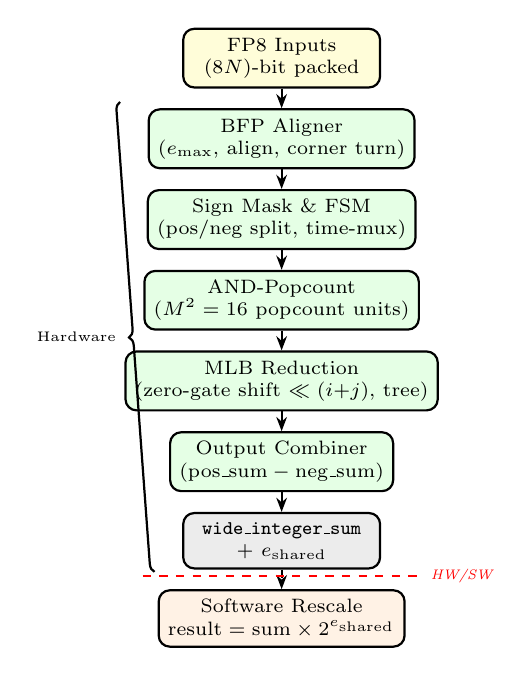
\begin{tikzpicture}[
  block/.style={draw, rounded corners, minimum width=2.5cm,
                minimum height=0.55cm, font=\scriptsize, align=center,
                thick},
  hw/.style={block, fill=green!10},
  sw/.style={block, fill=orange!10},
  arr/.style={-{Stealth[length=1.8mm]}, thick},
]
  \node[block, fill=yellow!15] (in) {FP8 Inputs\\$(8N)$-bit packed};
  \node[hw, below=0.25 of in] (bfp) {BFP Aligner\\($e_{\max}$, align, corner turn)};
  \node[hw, below=0.25 of bfp] (sign) {Sign Mask \& FSM\\(pos/neg split, time-mux)};
  \node[hw, below=0.25 of sign] (andpc) {AND-Popcount\\($M^2 = 16$ popcount units)};
  \node[hw, below=0.25 of andpc] (mlbred) {MLB Reduction\\(zero-gate shift $\ll (i{+}j)$, tree)};
  \node[hw, below=0.25 of mlbred] (comb) {Output Combiner\\($\text{pos\_sum} - \text{neg\_sum}$)};
  \node[block, fill=gray!15, below=0.25 of comb] (out) {\texttt{wide\_integer\_sum}\\+ $e_{\text{shared}}$};
  \node[sw, below=0.25 of out] (swrescale) {Software Rescale\\$\text{result} = \text{sum} \times 2^{e_{\text{shared}}}$};

  \draw[arr] (in) -- (bfp);
  \draw[arr] (bfp) -- (sign);
  \draw[arr] (sign) -- (andpc);
  \draw[arr] (andpc) -- (mlbred);
  \draw[arr] (mlbred) -- (comb);
  \draw[arr] (comb) -- (out);
  \draw[arr, dashed] (out) -- (swrescale);

  \draw[thick, red, dashed]
    ($(out.south west)+(-0.5,-0.08)$) -- ($(out.south east)+(0.5,-0.08)$)
    node[right, font=\tiny\itshape, red] {HW/SW};

  \draw[decorate, decoration={brace, amplitude=3pt, mirror}, thick]
    ($(bfp.north west)+(-0.35,0.08)$) -- ($(out.south west)+(-0.35,-0.03)$)
    node[midway, left=4pt, font=\tiny, align=center] {Hardware};
\end{tikzpicture}
}%
\caption{End-to-end pipeline of the proposed AND-popcount MLB-MAC
         accelerator with BFP front end.}
\label{fig:system}
\end{figure}

\subsection{Architecture~1: AND-Popcount MLB-MAC with BFP (Proposed)}
\label{ssec:mlb_arch}

The proposed architecture replaces all per-element multipliers with
bitwise AND gates and popcount trees.  It consists of four major
components, shown in Fig.~\ref{fig:mlb_arch}.

\textbf{BFP Aligner.}
A purely combinational module that takes an $(8N)$-bit packed FP8
vector as input.  In a first pass, it extracts the 4-bit exponent
from each lane and finds $e_{\max}$ across all $N$ lanes.  In a
second pass, for each lane it restores the hidden bit
($\text{mant} = \{1, m_2, m_1, m_0\}$ for $e \neq 0$; flushed to
zero for subnormals), right-shifts by $(e_{\max} - e_k)$ bits
(truncating), and performs a \emph{corner turn}: the $M$~bits of each
aligned mantissa are distributed across $M$~$N$-bit bit-planes.

\textbf{AND-Popcount Unit.}
For a pair of $N$-bit activation and weight bit-planes, an AND gate
array computes $\texttt{xnn}[k] = a[k] \mathbin{\&} b[k]$.  A
binary reduction tree sums these $N$ bits into a
$\text{PC}$-bit unsigned popcount
($\text{PC} = \lfloor \log_2 N \rfloor + 1$).

\textbf{MLB Unit (Zero-Gate Multiplier).}
Instantiates one AND-popcount and applies a static left-shift by
$(i+j)$ bit-positions, where $i$ and $j$ index the activation
and weight bit-planes.  Since $2^{i+j}$ is the product of the plane
weights $2^i \cdot 2^j$, this shift replaces what would otherwise
be a multiplier cell --- costing zero gates in hardware.

\textbf{MLB Array.}
An $M \times M$ grid of MLB units ($M^2 = 16$ for FP8).
Unit~$(i,j)$ receives activation plane~$i$ and weight plane~$j$
with shift amount~$i + j$.  The outputs feed a multi-level
combinational reduction tree producing a signed output.

\textbf{Sign-Handling FSM and Output Combiner.}
FP8 uses sign-magnitude representation.  Per-lane product signs
$s_k = s_{x,k} \oplus s_{w,k}$ partition lanes into positive and
negative groups via bitmask AND.  A 3-state FSM time-multiplexes
positive and negative activation planes through a \emph{single
shared} MLB array over two consecutive cycles, halving the array
instantiation count.  The output FSM catches both partial sums and
forms: $\texttt{result} = \text{pos\_sum} - \text{neg\_sum}$.

\begin{figure}[htbp]
\centering
\resizebox{0.38\textwidth}{!}{%
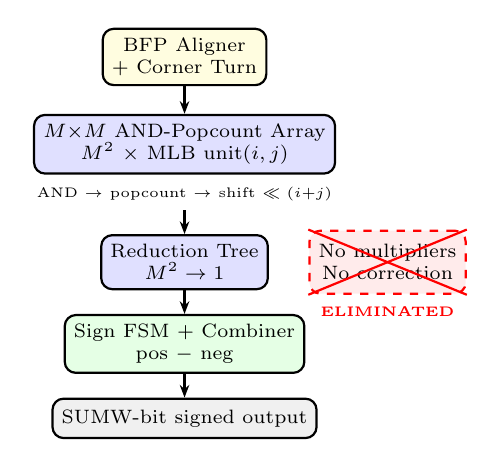
\begin{tikzpicture}[
  blk/.style={draw, thick, rounded corners, minimum width=1.8cm,
              minimum height=0.5cm, font=\scriptsize, align=center},
  core/.style={blk, fill=blue!12},
  arr/.style={-{Stealth[length=1.6mm]}, thick},
  lbl/.style={font=\tiny},
]
  \node[blk, fill=yellow!12] (bfp) {BFP Aligner\\+ Corner Turn};
  \node[core, below=0.35 of bfp, minimum width=3.5cm] (andpc)
    {$M{\times}M$ AND-Popcount Array\\$M^2$ $\times$ MLB unit$(i,j)$};
  \node[lbl, below=0.03 of andpc] (detail)
    {AND $\to$ popcount $\to$ shift $\ll (i{+}j)$};
  \node[core, below=0.3 of detail] (tree)
    {Reduction Tree\\$M^2 \to 1$};
  \node[blk, fill=green!10, below=0.3 of tree] (sign)
    {Sign FSM + Combiner\\pos $-$ neg};
  \node[blk, fill=gray!12, below=0.3 of sign] (outreg)
    {SUMW-bit signed output};

  \draw[arr] (bfp) -- (andpc);
  \draw[arr] (detail) -- (tree);
  \draw[arr] (tree) -- (sign);
  \draw[arr] (sign) -- (outreg);

  \node[blk, fill=red!8, draw=red, dashed, right=0.5 of tree,
        minimum width=1.6cm, minimum height=0.8cm] (nomul)
    {No multipliers\\No correction};
  \draw[red, thick] (nomul.north west) -- (nomul.south east);
  \draw[red, thick] (nomul.north east) -- (nomul.south west);
  \node[lbl, below=0.03 of nomul, red] {\textbf{ELIMINATED}};
\end{tikzpicture}
}%
\caption{Proposed AND-popcount MLB-MAC core (Architecture~1).}
\label{fig:mlb_arch}
\end{figure}

\subsection{Architecture~2: Integer MAC with BFP (Baseline~1)}
\label{ssec:int_arch}

To isolate the benefit of replacing multipliers with AND-popcount
logic, we implement a conventional integer MAC that uses the
\emph{same} BFP front end (Fig.~\ref{fig:int_arch}).  This ensures
that any difference in area and power is attributable solely to the
MAC core, not the exponent-handling strategy.

The integer MAC consists of three blocks:

\textit{Block~1 --- $N$ Parallel MAC Lanes.}
Each lane computes an unsigned $M \times M$-bit mantissa product,
applies the per-lane XOR sign to produce a signed product, and
accumulates into a signed register.

\textit{Block~2 --- Signed Reduction Tree.}
A binary adder tree reduces the $N$ signed accumulators to a
single sum.

\textit{Block~3 --- Scaling and Offset.}
An optional $\alpha_x \cdot \alpha_w$ multiplication and
$\beta_{xw}$ offset are applied.  For our comparison,
$\alpha_x = \alpha_w = 1$ and $\beta_{xw} = 0$.

The shared-exponent formula is identical to Eq.~(\ref{eq:shared_exp}).

\begin{figure}[htbp]
\centering
\resizebox{0.32\textwidth}{!}{%
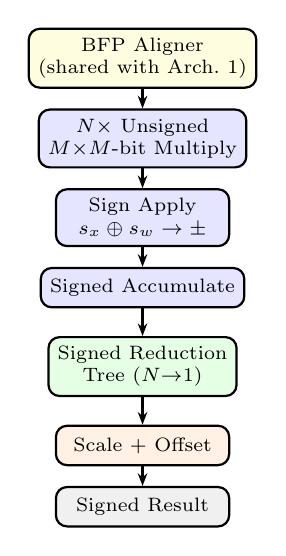
\begin{tikzpicture}[
  blk/.style={draw, thick, rounded corners, minimum width=2.2cm,
              minimum height=0.5cm, font=\scriptsize, align=center},
  b1/.style={blk, fill=blue!10},
  b2/.style={blk, fill=green!10},
  b3/.style={blk, fill=orange!10},
  arr/.style={-{Stealth[length=1.6mm]}, thick},
]
  \node[blk, fill=yellow!12] (bfp) {BFP Aligner\\(shared with Arch.~1)};
  \node[b1, below=0.25 of bfp] (mul) {$N \times$ Unsigned\\$M{\times}M$-bit Multiply};
  \node[b1, below=0.25 of mul] (sgn) {Sign Apply\\$s_x \oplus s_w \to \pm$};
  \node[b1, below=0.25 of sgn] (acc) {Signed Accumulate};
  \node[b2, below=0.35 of acc] (tree) {Signed Reduction\\Tree ($N {\to} 1$)};
  \node[b3, below=0.35 of tree] (scale) {Scale + Offset};
  \node[blk, fill=gray!12, below=0.25 of scale] (out) {Signed Result};

  \draw[arr] (bfp) -- (mul);
  \draw[arr] (mul) -- (sgn);
  \draw[arr] (sgn) -- (acc);
  \draw[arr] (acc) -- (tree);
  \draw[arr] (tree) -- (scale);
  \draw[arr] (scale) -- (out);
\end{tikzpicture}
}%
\caption{Integer MAC + BFP baseline (Architecture~2).}
\label{fig:int_arch}
\end{figure}

\subsection{Architecture~3: Native FP8 MAC (Baseline~2)}
\label{ssec:native_arch}

To quantify the full benefit of BFP exponent sharing, we implement
a native FP8 MAC that performs per-element floating-point
multiplication with no BFP blocking (Fig.~\ref{fig:native_arch}).
This represents the most hardware-expensive approach.

The native FP8 MAC operates in three stages:

\textit{Stage~1 --- $N$ Parallel FP8 Multipliers.}
Each lane independently: (a)~extracts sign, exponent, and mantissa;
(b)~restores the hidden bit (or adjusts for subnormals);
(c)~computes an unsigned mantissa product;
(d)~sums the two exponents;
(e)~aligns the product into a wide fixed-point field by
left-shifting by $(\text{exp\_sum} - 2)$ positions using a
per-element barrel shifter; and (f)~applies the product sign.

\textit{Stage~2 --- $N$-to-1 Signed Reduction Tree.}
A multi-level binary adder tree sums the $N$ signed products.

\textit{Stage~3 --- Output Register.}
The wide signed sum is registered, with an implicit fixed-point
scale.

The critical difference from the BFP-based architectures is that
\emph{every lane} requires its own barrel shifter with a wide shift
range, and the intermediate values are significantly wider before
reduction.  This per-element shifting is the dominant area and power
contributor that BFP amortizes.

\begin{figure}[htbp]
\centering
\resizebox{0.32\textwidth}{!}{%
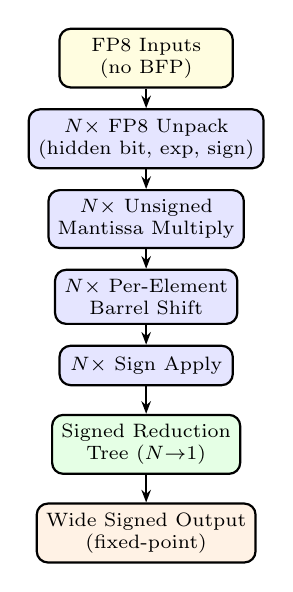
\begin{tikzpicture}[
  blk/.style={draw, thick, rounded corners, minimum width=2.2cm,
              minimum height=0.5cm, font=\scriptsize, align=center},
  s1/.style={blk, fill=blue!10},
  s2/.style={blk, fill=green!10},
  s3/.style={blk, fill=orange!10},
  arr/.style={-{Stealth[length=1.6mm]}, thick},
]
  \node[blk, fill=yellow!12] (in) {FP8 Inputs\\(no BFP)};
  \node[s1, below=0.25 of in] (unp) {$N \times$ FP8 Unpack\\(hidden bit, exp, sign)};
  \node[s1, below=0.25 of unp] (mul) {$N \times$ Unsigned\\Mantissa Multiply};
  \node[s1, below=0.25 of mul] (shift) {$N \times$ Per-Element\\Barrel Shift};
  \node[s1, below=0.25 of shift] (sgn) {$N \times$ Sign Apply};
  \node[s2, below=0.35 of sgn] (tree) {Signed Reduction\\Tree ($N {\to} 1$)};
  \node[s3, below=0.35 of tree] (out) {Wide Signed Output\\(fixed-point)};

  \draw[arr] (in) -- (unp);
  \draw[arr] (unp) -- (mul);
  \draw[arr] (mul) -- (shift);
  \draw[arr] (shift) -- (sgn);
  \draw[arr] (sgn) -- (tree);
  \draw[arr] (tree) -- (out);
\end{tikzpicture}
}%
\caption{Native FP8 MAC baseline (Architecture~3, no BFP).}
\label{fig:native_arch}
\end{figure}

\subsection{Three-Way Architectural Comparison}
\label{ssec:comparison}

Table~\ref{tab:3way} summarises the key structural differences
between the three architectures.

\begin{table}[htbp]
\centering
\caption{Structural comparison of the three FP8 dot-product
architectures ($M = 4$ bit-planes).}
\label{tab:3way}
\footnotesize
\begin{tabular}{lccc}
\toprule
Component & \textbf{AND-Pop.} & \textbf{INT MAC} & \textbf{Native} \\
          & \textbf{MLB+BFP} & \textbf{+BFP}   & \textbf{FP8 MAC} \\
\midrule
BFP front end        & Yes  & Yes  & No  \\
Per-element multiply & None (AND) & $M{\times}M$-bit & $M{\times}M$-bit \\
Per-element shift    & None & None & Wide barrel \\
Popcount trees ($M^2$) & Yes  & None & None \\
Correction circuit   & None & None & N/A \\
Sign handling        & Time-muxed & Per-lane & Per-lane \\
MLB array instances  & 1 (shared) & N/A & N/A \\
\bottomrule
\end{tabular}
\end{table}

\subsection{Parameterizable Bit-Width Formulas}
\label{ssec:bitwidths}

All module bit widths for the proposed AND-popcount MLB-MAC are
derived from the parallelism factor~$N$:
\begin{align}
    \text{PC} &= \lfloor \log_2 N \rfloor + 1
    & &\text{(popcount bits)}, \label{eq:pc} \\
    \text{UNITW} &= \text{PC} + 2M + 1
    & &\text{(MLB unit output)}, \label{eq:unitw} \\
    \text{MLBW} &= \text{UNITW} + M
    & &\text{(MLB array output)}, \label{eq:mlbw} \\
    \text{SUMW} &= \text{MLBW} + 1
    & &\text{(final output)}, \label{eq:sumw}
\end{align}
with input bus width $\text{VW} = 8N$ and plane bus width
$\text{PW} = MN$.  Table~\ref{tab:bitwidths} lists concrete
values for $M = 4$.

\begin{table}[htbp]
\centering
\caption{Bit widths for the AND-popcount MLB-MAC at each $N$ ($M=4$).}
\label{tab:bitwidths}
\footnotesize
\begin{tabular}{rrrrrr}
\toprule
$N$ & PC & UNITW & MLBW & SUMW & VW \\
\midrule
9   & 4  & 13   & 17  & 18  & 72  \\
25  & 5  & 14   & 18  & 19  & 200 \\
32  & 6  & 15   & 19  & 20  & 256 \\
64  & 7  & 16   & 20  & 21  & 512 \\
128 & 8  & 17   & 21  & 22  & 1024 \\
256 & 9  & 18   & 22  & 23  & 2048 \\
512 & 10 & 19   & 23  & 24  & 4096 \\
\bottomrule
\end{tabular}
\end{table}

% =========================================================================
\section{Software Verification: Bit-Accurate PyTorch Emulator}
% =========================================================================
\label{sec:pytorch}

To validate the hardware design and characterise accuracy
trade-offs, we develop a bit-accurate PyTorch emulator that
mirrors the RTL pipeline at every stage.  The emulator
provides three models:

\begin{itemize}
    \item An \textbf{MLB-BFP model} that performs FP8 quantisation,
    BFP alignment with corner turn, and the full AND-popcount
    dot-product simulation (matching Architecture~1).
    \item An \textbf{FP8 baseline model} that quantises to FP8
    and performs standard matrix multiplication without BFP
    blocking (matching Architecture~3).
    \item A \textbf{full-precision model} for reference.
\end{itemize}

The FP8 quantiser implements the E4M3 encode--decode cycle: clamp,
extract biased exponent and 3-bit mantissa, reconstruct, and flush
subnormals to zero.  The backward pass uses a Straight-Through
Estimator~(STE)~\cite{b_ste} that passes gradients unchanged.

The BFP alignment step mirrors the hardware exactly: find
$e_{\max}$ per block, restore hidden bits, right-shift by
$\Delta e_k$ using integer-truncating division, and corner-turn
into $M$ bit-planes.  An exponent-sorted permutation option
clusters values of similar magnitude into the same block by
sorting the inner-product dimension by mean weight exponent before
chunking, reducing per-block exponent spread.

The test network is ResNet-20 for CIFAR-10~\cite{b_resnet} ($32
\times 32$ RGB images, 50K/10K split, standard augmentation).
The QAT sweep operates in two phases:

\textbf{Phase~1 --- FP8 Baseline:} The FP8 model is trained for
20~epochs (SGD, batch size~128, learning rate~0.1) to establish a
baseline checkpoint.

\textbf{Phase~2 --- QAT Fine-Tuning:} For each
$N \in \{9, 25, 32, 64, 128, 256, 512\}$, a fresh model with
MLB-BFP layers is initialised from the Phase~1 checkpoint and
fine-tuned for 30~epochs (SGD, learning rate~0.01, cosine
annealing).  The best test accuracy per $N$ is recorded.

% =========================================================================
\section{Experimental Setup}
% =========================================================================
\label{sec:experimental}

All three architectures were implemented, tested, and verified in
Verilog.  A standard synthesis tool was utilised for logic
synthesis and performance analysis, producing precise power
consumption estimates, area utilisation, and timing
characteristics.  The physical design targeted the 45\,nm
technology node using the FreePDK45 library, offering a good
balance between performance and power efficiency.  All three
architectures were synthesised with the same library and
constraints to ensure a fair comparison.

Each architecture was verified by a self-checking testbench
containing 11~directed corner cases and 50~pseudorandom tests
(61~total per $N$ value).  A behavioural reference model within
the testbench mirrors the hardware algorithm exactly and compares
outputs bit-for-bit.

% =========================================================================
\section{Results}
% =========================================================================
\label{sec:results}

\subsection{Synthesis: Area Comparison}

Table~\ref{tab:area} compares the synthesised cell area of all three
architectures, normalised to the native FP8 MAC baseline.

\begin{table}[htbp]
\centering
\caption{Synthesised cell area comparison
(FreePDK45, 45\,nm).}
\label{tab:area}
\begin{tabular}{lcc}
\toprule
Architecture & Area ($\mu\text{m}^2$) & Normalised \\
\midrule
Native FP8 MAC (no BFP)    & TBD & 1.00 \\
INT MAC + BFP (Baseline~1) & TBD & TBD \\
AND-Pop.\ MLB + BFP (Proposed) & TBD & TBD \\
\bottomrule
\end{tabular}
\end{table}

\subsection{Synthesis: Power Comparison}

Table~\ref{tab:power} compares the total power (dynamic + leakage).

\begin{table}[htbp]
\centering
\caption{Power comparison
(FreePDK45, 45\,nm).}
\label{tab:power}
\begin{tabular}{lcc}
\toprule
Architecture & Power (mW) & Normalised \\
\midrule
Native FP8 MAC (no BFP)    & TBD & 1.00 \\
INT MAC + BFP (Baseline~1) & TBD & TBD \\
AND-Pop.\ MLB + BFP (Proposed) & TBD & TBD \\
\bottomrule
\end{tabular}
\end{table}

% Placeholder: Area and power breakdown plots (similar to [1] Fig. 8-9)
% will replace these tables once synthesis data is collected.

\subsection{RTL Functional Verification}

Table~\ref{tab:verification} summarises the testbench results.
All architectures achieve 100\% pass rates across all 61 test
vectors per $N$, confirming bit-exact agreement with the
behavioural reference model.

\begin{table}[htbp]
\centering
\caption{Functional verification results: pass rate per $N$.}
\label{tab:verification}
\footnotesize
\begin{tabular}{rcccc}
\toprule
$N$ & \multicolumn{2}{c}{AND-Popcount MLB} &
      \multicolumn{2}{c}{INT MAC + BFP} \\
\cmidrule(lr){2-3} \cmidrule(lr){4-5}
& Directed & Random & Directed & Random \\
\midrule
9   & 11/11 & 50/50 & 11/11 & 50/50 \\
25  & 11/11 & 50/50 & 11/11 & 50/50 \\
32  & 11/11 & 50/50 & 11/11 & 50/50 \\
64  & 11/11 & 50/50 & 11/11 & 50/50 \\
128 & 11/11 & 50/50 & 11/11 & 50/50 \\
256 & 11/11 & 50/50 & 11/11 & 50/50 \\
512 & 11/11 & 50/50 & 11/11 & 50/50 \\
\bottomrule
\end{tabular}
\end{table}

\subsection{QAT Accuracy vs.\ Block Size}
\label{ssec:qat_results}

Table~\ref{tab:qat} shows ResNet-20 top-1 accuracy on CIFAR-10
as a function of BFP block size $N$, after QAT fine-tuning from
the FP8 baseline.  Exponent-sorted blocking is enabled for all
runs.  Both BFP-based architectures (proposed and INT MAC baseline)
produce \emph{identical} accuracy at each $N$, since they compute
the same mathematical function; the difference is only in hardware
cost.

\begin{table}[htbp]
\centering
\caption{ResNet-20/CIFAR-10 top-1 accuracy vs.\ BFP block size $N$
         (QAT fine-tuning, exponent-sorted blocking).}
\label{tab:qat}
\begin{tabular}{lcc}
\toprule
Block size $N$ & Top-1 Acc.\ (\%) & $\Delta$ vs.\ FP8 (pp) \\
\midrule
FP8 baseline (no BFP) & TBD & 0.0 \\
\midrule
9   & TBD & TBD \\
25  & TBD & TBD \\
32  & TBD & TBD \\
64  & TBD & TBD \\
128 & TBD & TBD \\
256 & TBD & TBD \\
512 & TBD & TBD \\
\bottomrule
\end{tabular}
\end{table}

% =========================================================================
\section{Discussion}
% =========================================================================

\textbf{Why AND-popcount MLB saves area and power.}
The proposed architecture eliminates the two most expensive
components in a conventional FP8 MAC array:
(1)~Per-element multipliers --- replaced by $N$-wide AND gates
and $\lceil\log_2 N\rceil$-depth popcount trees.
(2)~Per-element barrel shifters --- the BFP front end reduces
all $N$ lanes to a shared exponent using fixed-width right shifts,
in contrast to the native FP8 MAC which requires wide per-element
barrel shifters.  The BFP alignment cost is amortized across the
entire block and shared between the proposed design and the INT
MAC baseline.

\textbf{AND-popcount is correction-free for FP8.}
Prior MLB-MAC work~\cite{b1} used XNOR-popcount, which
requires correction circuits when applied to unsigned data.  Our
initial XNOR implementation confirmed that this correction overhead
consumed enough area to partially negate the benefit of eliminating
multipliers.  The AND-popcount approach avoids this entirely because
FP8 mantissa bits are natively unsigned ---
$\text{AND}(x_i, x_j) = x_i \cdot x_j$ with no offset.
The correction terms are \emph{mathematically zero}, not merely
small.

\textbf{The zero-gate multiplier.}
Each MLB unit scales the popcount by $2^{i+j}$.  Since this is a
power of two, it is implemented as a static wire-shift, costing
zero gates.  In contrast, the XNOR design required a per-unit
LUT-based multiplier module --- all $M^2$ instances eliminated.

\textbf{BFP vs.\ native FP8: the exponent trade-off.}
The native FP8 MAC preserves full per-element exponent precision
but pays for it with $N$ individual barrel shifters and wide
intermediate values.  The BFP-based architectures replace this
with a single shared exponent and $M$-bit aligned mantissas,
dramatically reducing datapath width and shifter complexity.  The
trade-off is precision loss at large $N$; our QAT sweep with
exponent-sorted blocking quantifies this.

\textbf{$K/N$ trade-off.}
Following the analysis in~\cite{b1}, when the dot-product size $K$
exceeds~$N$, the result is computed as $\lceil K/N \rceil$
independent BFP-MLB passes.  The reduction and BFP-alignment
overhead is amortized as $K/N$ grows, improving the relative
efficiency of the MLB approach.  Conversely, when $K < N$, the
inputs are zero-padded, leading to under-utilisation.  The optimal
$N$ depends on the typical $K$ values in the target network.

\textbf{Accuracy equivalence of the two BFP-based architectures.}
Both BFP-based architectures compute \emph{mathematically identical}
dot products.  The accuracy numbers in Table~\ref{tab:qat} apply
equally to both.  The advantage of the proposed design is purely
in hardware cost (area, power), not accuracy.

\textbf{Functional verification confidence.}
The 61-vector testbench covers all critical corner cases.  The
behavioural reference model is algebraically identical to the
PyTorch emulator, establishing a three-way equivalence: PyTorch
model $\leftrightarrow$ Verilog reference $\leftrightarrow$
Verilog RTL.

% =========================================================================
\section{Conclusion}
% =========================================================================

We have presented an energy-efficient FP8 dot-product accelerator
that replaces conventional multiplier arrays with AND gates and
popcount reduction trees, combined with a Block Floating Point
front end for exponent sharing.  The design exploits the unsigned
mantissa structure of the FP8~(E4M3) format to make AND-popcount
correction-free, unlike prior XNOR-based MLB approaches that
required substantial correction circuitry.

We compared three FP8 dot-product architectures: (1)~the proposed
AND-popcount MLB-MAC with BFP, (2)~a conventional integer MAC
with the same BFP front end, and (3)~a native FP8 MAC without BFP.
All designs are synthesised on the 45\,nm node using the FreePDK45
library and verified bit-exactly across 61 test vectors per block
size~$N$.
A QAT sweep on ResNet-20/CIFAR-10 with exponent-sorted blocking
characterises the accuracy--area trade-off for selecting the
optimal block size.

\section*{Acknowledgment}

The authors thank the IIIT Bangalore VLSI and Systems group for
compute resources and technical discussions.

\begin{thebibliography}{00}
\bibitem{b1}
    A.~Ansarmohammadi, R.~Hojabr, M.~Mastalizade, N.~Nazari, and
    M.~E.~Salehi,
    ``MLB-MAC: Multi-Level Binary MAC Array for Energy Efficient ML
    Accelerators,''
    \textit{IEEE Trans.\ Circuits Syst.\ I}, vol.~72, no.~10,
    pp.~5657--5670, Oct.\ 2025.

\bibitem{b2}
    P.~Micikevicius \textit{et al.},
    ``FP8 Formats for Deep Learning,''
    \textit{arXiv preprint arXiv:2209.05433}, 2022.

\bibitem{b3}
    S.~Rouhani \textit{et al.},
    ``Microscaling Data Formats for Deep Learning,''
    \textit{arXiv preprint arXiv:2310.10537}, 2023.

\bibitem{b_ste}
    Y.~Bengio, N.~L{\'e}onard, and A.~Courville,
    ``Estimating or Propagating Gradients Through Stochastic
    Neurons for Conditional Computation,''
    \textit{arXiv preprint arXiv:1308.3432}, 2013.

\bibitem{b_resnet}
    K.~He, X.~Zhang, S.~Ren, and J.~Sun,
    ``Deep Residual Learning for Image Recognition,''
    in \textit{Proc.\ IEEE CVPR}, 2016, pp.~770--778.

\end{thebibliography}

\end{document}
